\documentclass[11pt,a4paper]{article}
\usepackage[spanish,es-nodecimaldot]{babel}	% Utilizar español
\usepackage[utf8]{inputenc}					% Caracteres UTF-8
\usepackage{graphicx}						% Imagenes
\usepackage[hidelinks]{hyperref}			% Poner enlaces sin marcarlos en rojo
\usepackage{fancyhdr}						% Modificar encabezados y pies de pagina
\usepackage{float}							% Insertar figuras
\usepackage[textwidth=390pt]{geometry}		% Anchura de la pagina
\usepackage[nottoc]{tocbibind}				% Referencias (no incluir num pagina indice en Indice)
\usepackage{enumitem}						% Permitir enumerate con distintos simbolos
\usepackage[T1]{fontenc}					% Usar textsc en sections
\usepackage{amsmath}						% Símbolos matemáticos
\usepackage{natbib}
\usepackage{subcaption}

% Comando para poner el nombre de la asignatura
\newcommand{\asignatura}{Visión por Computador}
\newcommand{\autor}{Vladislav Nikolov Vasilev}
\newcommand{\titulo}{Práctica 2}
\newcommand{\subtitulo}{Redes Neuronales Convolucionales}

\usepackage{listings}
\usepackage{xcolor}
 
\definecolor{codegreen}{rgb}{0,0.6,0}
\definecolor{codegray}{rgb}{0.5,0.5,0.5}
\definecolor{codepurple}{rgb}{0.58,0,0.82}
\definecolor{backcolour}{rgb}{0.95,0.95,0.92}
 
\lstdefinestyle{mystyle}{
    backgroundcolor=\color{backcolour},   
    commentstyle=\color{codegreen},
    keywordstyle=\color{magenta},
    numberstyle=\tiny\color{codegray},
    stringstyle=\color{codepurple},
    basicstyle=\ttfamily\footnotesize,
    breakatwhitespace=false,         
    breaklines=true,                 
    captionpos=b,                    
    keepspaces=true,                 
    numbers=left,                    
    numbersep=5pt,                  
    showspaces=false,                
    showstringspaces=false,
    showtabs=false,                  
    tabsize=4,
    language=Python,
    literate={ñ}{{\~n}}1
}

\lstset{style=mystyle}

% Configuracion de encabezados y pies de pagina
\pagestyle{fancy}
\lhead{\autor{}}
\rhead{\asignatura{}}
\lfoot{Grado en Ingeniería Informática}
\cfoot{}
\rfoot{\thepage}
\renewcommand{\headrulewidth}{0.4pt}		% Linea cabeza de pagina
\renewcommand{\footrulewidth}{0.4pt}		% Linea pie de pagina


\begin{document}
\pagenumbering{gobble}

% Pagina de titulo
\begin{titlepage}

\begin{minipage}{\textwidth}

\centering


\includegraphics[scale=0.5]{img/ugr.png}\\

\textsc{\Large \asignatura{}\\[0.2cm]}
\textsc{GRADO EN INGENIERÍA INFORMÁTICA}\\[1cm]

\noindent\rule[-1ex]{\textwidth}{1pt}\\[1.5ex]
\textsc{{\Huge \titulo\\[0.5ex]}}
\textsc{{\Large \subtitulo\\}}
\noindent\rule[-1ex]{\textwidth}{2pt}\\[3.5ex]

\end{minipage}

\vspace{0.5cm}

\begin{minipage}{\textwidth}

\centering

\textbf{Autor}\\ {\autor{}}\\[2.5ex]
\textbf{Rama}\\ {Computación y Sistemas Inteligentes}\\[2.5ex]
\vspace{0.3cm}


\includegraphics[scale=0.3]{img/etsiit.jpeg}

\vspace{0.7cm}
\textsc{Escuela Técnica Superior de Ingenierías Informática y de Telecomunicación}\\
\vspace{1cm}
\textsc{Curso 2019-2020}
\end{minipage}
\end{titlepage}

\pagenumbering{arabic}
\tableofcontents
\thispagestyle{empty}				% No usar estilo en la pagina de indice

\newpage

\setlength{\parskip}{1em}

\section{\textsc{BaseNet en CIFAR100}}

Antes de empezar con la traducción de la arquitectura proporcionada de \textit{BaseNet}, hace falta establecer la forma
de la entrada de la primera capa de la red. Esto es necesario, ya que el modelo necesita conocer dicho tamaño para poder
ser compilado sin ningún tipo de error. Como las imágenes de \textit{CIFAR100} tienen un tamaño de $32 \times 32$
píxels, y tienen 3 canales, la dimensión de la entrada va a ser la siguiente:

\begin{lstlisting}
# Tamaño de la entrada
input_shape = (32, 32, 3)
\end{lstlisting}

Una vez definida la forma de la entrada, ya se puede empezar a hacer la traducción a código. El resultado es el siguiente:

\begin{lstlisting}
# Creacion del modelo
model = Sequential()
model.add(Conv2D(6, kernel_size=(5, 5), padding='valid',
				 input_shape=input_shape))
model.add(Activation('relu'))
model.add(MaxPooling2D(pool_size=(2, 2)))

model.add(Conv2D(16, kernel_size=(5, 5), padding='valid'))
model.add(Activation('relu'))
model.add(MaxPooling2D(pool_size=(2, 2)))

model.add(Flatten())
model.add(Dense(units=50))
model.add(Activation('relu'))
model.add(Dense(units=25))
model.add(Activation('softmax'))
\end{lstlisting}

BaseNet es un modelo secuencial, así que empezamos indicando eso. A continuación, añadimos el primer módulo convolucional.
Este se compone de una convolución 2D con un \textit{kernel} de $5 \times 5$, una función de activación no lineal (RELU en
este caso) y un MaxPooling de tamaño $2 \times 2$. El parámetro $padding = valid$ de $Conv2D$ indica que solo se tiene que
aplicar la convolución allá donde se pueda ajustar el \textit{kernel}; es decir, como en las regiones de los bordes no se
puede, se van a ignorar estas zonas, lo cuál implica que la salida no va a tener el mismo tamaño que la entrada. Este módulo
convolucional se repite otra vez. Después de eso, nos encontramos con las capas densas, las cuáles van a actuar como
clasificador. La capa $Flatten$ es necesario ponerla, ya que coge la salida de la anterior, la cuál es un bloque de tamaño
$5 \times 5 \times 16$ (16 imágenes $5 \times 5$), y aplana dicho bloque, convirtiéndolo en un vector de 400 características,
el cuál sirve como entrada al modelo denso. La última capa, la de activación \textit{softmax} es la que va a dar la salida,
un vector de probabilidades para cada clase. En este caso, la salida va a ser un vector de 25 posiciones, ya que estamos
en un problema donde hay 25 clases.

Con el modelo ya definido, y antes de compilarlo, tenemos que establecer algunas cosas más:

\begin{itemize}
	\item \textbf{Optimizador}. El optimizador que se va a utilizar en este caso es el \textbf{SGD} o \textit{Stochastic
	Gradient Descent}. 	Este es uno de los optimizadores más populares e importantes dentro del \textit{machine learning}.
	Se utiliza mucho con redes neuronales, ya sean redes normales o profundas, y es conocido por su robustez y por ofrecer
	unos muy buenos resultados	en general, además de ser bastante rápido a diferencia de otros optimizadores, como por ejemplo
	Adam. En este caso, se va a utilizar con los parámetros por defecto. Es decir, se tendrá un \textit{learning rate} de 0.01,
	y no se utilizará momentum ni el momentum de Nesterov. Estos parámetros parecen razonables, ya que el \textit{learning
	rate} no es ni demasaido pequeño ni demasiado grande. Además, como es un poco difícil ajustar el momento, se ha preferido
	no tocar este parámetro.
	\item \textbf{Tamaño del \textit{batch}}. Otro elemento muy importante a determinar es el tamaño del \textit{batch}, si bien
	no es necesario conocerlo en el momento en el que se compila el modelo. Para un problema como este, teniendo en cuenta que
	tenemos unos 11250 datos de entrenamiento, un tamaño de \textit{batch} razonable es de 32. Este es un tamaño muy utilizado,
	ya que en general ofrece unos buenos resultados, ya que permite converger a buenos óptimos y hace que el modelo
	generalice bastante bien. Con un tamaño menor se estaría explorando demasiado el espacio, mientras que con uno mayor se
	estaría explotando una zona del espacio, lo cuál puede llegar a producir problemas, como que no se generalice demasiado
	bien \cite{DBLP:journals/corr/KeskarMNST16}, cosa que no nos interesa.
	\item \textbf{Número de épocas}. Éste es quizás el parámetro más difícil de decidir a priori, ya que no tenemos mucha
	información. Por tanto, ya que a medida que vayamos haciendo pruebas podremos ver las curvas de entrenamiento y validación,
	podremos decidir en función de éstas cuántas épocas debemos entrenar los modelos. Para empezar, podemos fijar unas 30 épocas,
	ya que parece un número razonable.
\end{itemize}

Con esto ya visto, podemos compilar nuestro modelo. Lo primero que tenemos que hacer es definir el optimizador. Como vamos
a utilizar SGD, lo hacemos de la siguiente forma:

\begin{lstlisting}
# Establecer optimizador a utilizar
optimizer = SGD()
\end{lstlisting}

Para compilar el modelo, lo haremos de la siguiente forma:

\begin{lstlisting}
# Compilar el modelo
model.compile(
    loss=keras.losses.categorical_crossentropy,
    optimizer=optimizer,
    metrics=['accuracy']
)
\end{lstlisting}

Como estamos en un problema de clasificación y la salida que va a dar el modelo es un vector de probabilidades para múltiples
clases, especificamos que la función de pérdida que se utilizará es la entropía cruzada o \textit{Categorical Cross-Entropy},
la cuál es muy utilizada en problemas de clasificación para múltples clases. Especificamos también cuál será el optimizador
a utilizar, e indicamos que la métrica que nos interesa es la precisión o \textit{accuracy}, que representa la proporción
de aciertos sobre el número total de elementos. Existen muchas otras métricas que se pueden utilizar, pero la \textit{accuracy}
es la más sencilla de entender.

Con el modelo ya compilado, podemos visualizarlo de la siguiente forma:

\begin{figure}[H]
  \centering
  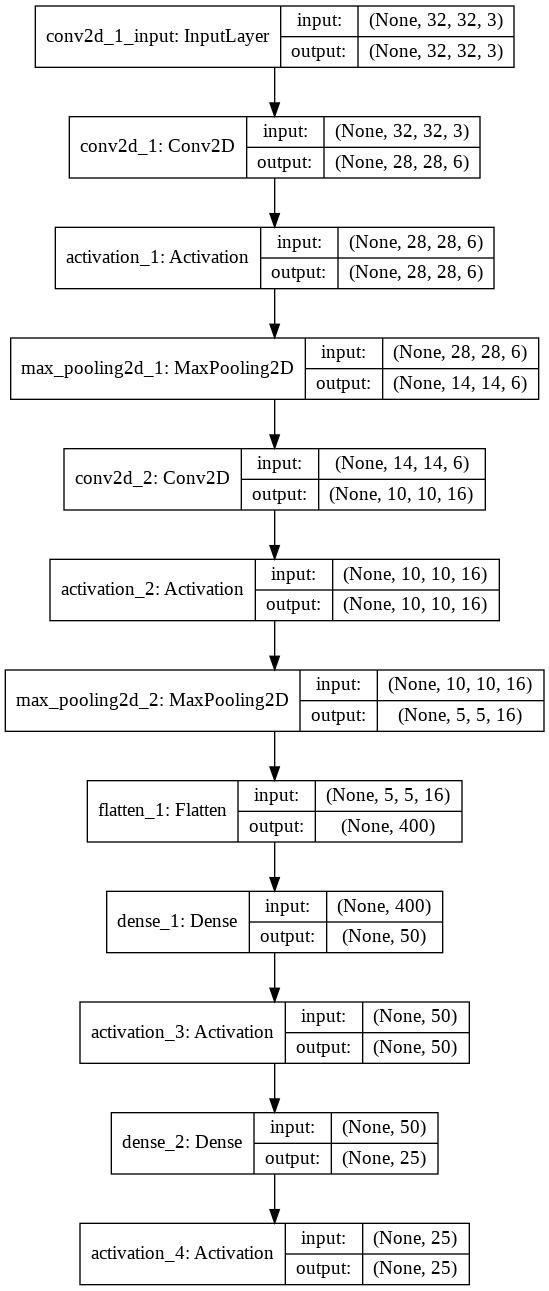
\includegraphics[scale=0.28]{img/base-model.png}
  \caption{Esquema que representa el modelo \textit{BaseNet}.}
  \label{fig:base-model}
\end{figure}

Aquí es donde podemos ver mejor la estructura del modelo. Se puede ver de forma más clara que antes la estructua secuencial
que tiene, además de cada una de las capas y de los tamaños de las entradas y de las salidas de éstas.

Teniendo el modelo ya construido y compilado, para hacernos una idea de como de bueno es, podemos entrenarlo y probarlo
con el conjunto de test. Es muy importante, antes de empezar, guardar los pesos que tiene el modelo. De esta forma, podremos
restablecerlos posteriormente, para poder reentrenar el modelo. Para guardar los pesos, podemos hacerlo de la siguiente
forma:

\begin{lstlisting}
# Guardar los pesos iniciales del modelo
weights = model.get_weights()
\end{lstlisting}

Ahora ya podemos proceder al entrenamiento. Es muy importante destacar que, con los datos de entrenamiento de los que disponemos,
solo se tiene que entrenar con el 90\% de éstos; el 10\% restante se tiene que dejar para validar el modelo, y de esta forma poder
obtener unas gráficas para el error y la \textit{accuracy} en los conjuntos de entrenamiento y de validación. Estos
valores que se obtienen para el conjunto de validación son, en general, una buena aproximación de lo que se puede obtener
en el conjunto de test, si la muestra es lo suficientemente representativa de la población total, claro está.

Para entrenar el modelo, lo hacemos de la siguiente forma:

\begin{lstlisting}
# Entrenar el modelo
history = model.fit(
    x_train,
    y_train,
    validation_split=0.1,
    epochs=epochs,
    batch_size=batch_size,
    verbose=1
)
\end{lstlisting}

Especificamos que se utilizan las particiones de entrenamiento $x\_train$ (las imágenes) e $y\_train$ (la etiqueta asociada
a cada una de las imágenes del conjunto de entrenamiento). Además, con $validation\_split = 0.1$ indicamos que solo el
10\% de los datos se utilizarán para validar el modelo. Se especifica también el tamaño del \textit{batch} (recordemos que
lo habíamos fijado a 32) y el número de épocas (30 inicialmente). El parámetro $verbose$ es solo para mostrar el progreso
del entrenamiento; no tiene ningún otro fin.

Este método devuelve una historia, la cuál se almacena en la variable $history$. Esta historia contiene trazas de la evolución
de los valores de la función de pérdida y de \textit{accuracy} en los conjuntos de entrenamiento y de validación.
Para este caso, hemos obtenido los siguientes resultados:

\begin{figure}[H]
  \centering
  \begin{subfigure}[t]{0.5\textwidth}
    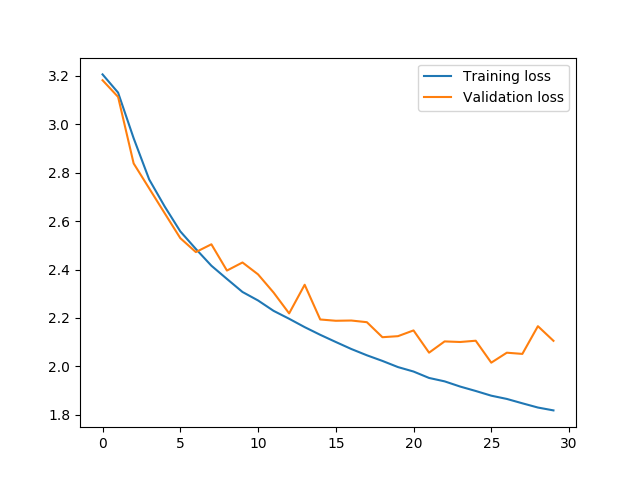
\includegraphics[scale=0.42]{img/base-model-loss.png}
    \caption{Evolución de la función de pérdida.}
    \label{fig:base-model-loss}
  \end{subfigure}%
  ~ \quad
  \begin{subfigure}[t]{0.5\textwidth}
    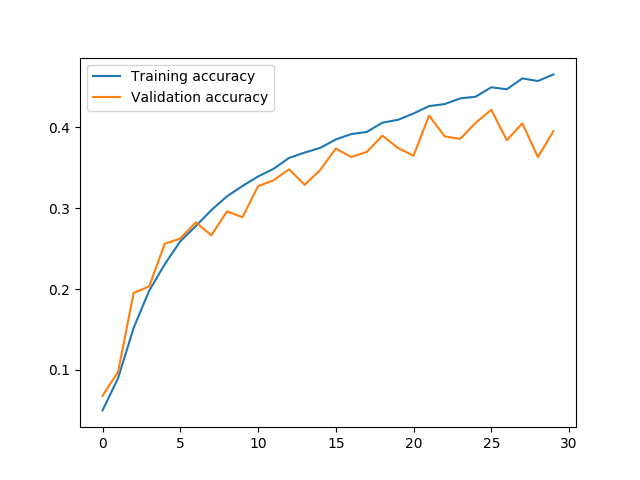
\includegraphics[scale=0.42]{img/base-model-acc.png}
    \caption{Evolución de la \textit{accuracy}.}
    \label{fig:base-model-acc}
  \end{subfigure}
  \caption{Historia del modelo \textit{BaseNet}.}
  \label{fig:basenet-history}
\end{figure}

Podemos ver que no se produce \textit{overfit}, ya que a medida que el valor del error o de la función de pérdida va
bajando en el conjunto de entrenamiento, también lo hace en el de validación, hasta que llega a las últimas épocas, donde dicho
valor se queda más o menos se queda un poco por encima del de entrenamiento, pareciendo que se estanca.
En ningún momento el error en validación llega a subir. Si esto hubiese sucedido, podríamos haber afirmado de forma clara
que se ha producido \textit{overfit} en nuestro modelo. Si miramos también la \textit{accuracy}, podemos ver que, a medida
que va subiendo dicho valor en el conjunto de entrenamiento, también lo hace en el de validación.
Aquí de nuevo sucede algo como en el caso de la función de pérdida, ya que parece que en las últimas épocas este valor se va
quedando un poco estancado, aunque no dista mucho del valor obtenido en el conjunto de entrenamiento.

Sin embargo, aunque el modelo no padezca de \textit{overfit}, sí que lo hace de \textit{underfit}: la evolución de los valores
de la función de pérdida y de la \textit{accuracy}, aunque en un principio parecen buenos ya que el error va disminuyendo y la
precisión aumentando, no es del todo satisfactoria. Podemos ver claramente como el error, aún en el conjunto de entrenamiento,
sigue siendo bastante alto (en las últimas épocas se queda en torno a $1.8$, valor bastante alto), y en el caso de la
precisión se queda en torno a $0.45$. En el caso del conjunto de validación, aunque al principio los valores sean más o
menos parejos con el conjunto de entrenamiento en ambas gráficas, podemos ver como al cabo de aproximadamente unas 15-20 épocas
los valores empiezan a ser dispares. En el caso de la función de pérdida, al final, los valores que se obtienen están en torno a 2,
mientras que en la precisión los valores obtenidos no superan el $0.4$, quedándose por debajo de los obtenidos en entrenamiento.

En líneas generales, estos resultados son demasiado pobres: lo ideal hubiese sido alcanzar un error cercano a 1 o
más bajo y una precisión superior a 0.5 en el conjunto de entrenamiento, y que los valores obtenidos en el conjunto de
validación hubiesen seguido casi perfectamente a los de entrenamiento. Por tanto, de aquí podemos extraer que todavía
existe mucho margen de mejora.

Es importante destacar, antes de continuar, que todos los resultados que se obtienen dependen de la ejecución. Es decir,
que para dos ejecuciones puede que los resultados no sean exactamente los mismos; sin embargo, podemos decir que estarán
bastante cerca, en general, ya que los datos son los mismos.

Para tener una idea de cómo de bien funciona nuestro modelo base con el conjunto de test, y para tener un valor de
\textit{accuracy} que podemos utilizar para comparar este modelo base con las mejoras futuras, vamos a hacer que prediga
las etiquetas del conjunto $x\_test$ (las imágenes de test), y compararemos dichos valores con los reales, los cuáles están
en la variable $y\_test$. Para hacer dicha predición, podemos hacerla de la siguiente forma:

\begin{lstlisting}
# Predecir los datos
prediction = model.predict(
    x_test,
    batch_size=batch_size,
    verbose=1
)
\end{lstlisting}

De esta forma, especificamos que el modelo prediga las etiquetas asociadas al conjunto $x\_test$ y se le especifica un tamaño
de \textit{batch}, que será el número de elementos máximos que se predigan de golpe; es decir, no se va mandar a CPU/GPU un
conjunto de datos de mayor tamaño que el especificado. El parámetro $verbose$ es, de nuevo, para mostrar el proceso.

El valor de \textit{accuracy} comparando los valores predichos con los reales gira en torno a $0.4$ tras realizar
algunas pruebas. Dicho valor, a pesar de no ser del todo horrible para un modelo tan simple, es bastante bajo, y creemos
que tiene cierto margen de mejora. ya que posiblemente, con realizar algunas modificaciones, podamos llegar una \textit{accuracy}
igual o superior a $0.5$. Por tanto, vamos a intentar mejorar nuestro modelo en la próxma sección,
para ver hasta dónde somos capaces de llegar.

\section{\textsc{Mejora del modelo}}

En esta sección, vamos a ir proponiendo una serie de mejoras que podemos hacer sobre el modelo. Estas mejoras son acumulativas,
es decir, que se van realizando una sobre la otra, siempre y cuando ofrezcan unos buenos resultados.

Para cada caso, vamos a discutir brevemente qué es lo que se va a mejorar, qué parámetros se van a utilizar y cuáles son los
resultados obtenidos. Para cada experimento mostraremos gráficas, iguál que las que se pueden ver en la figura
\ref{fig:basenet-history}.

Una vez que hayamos encontrado un modelo bueno (es decir, uno que no sufre ni de \textit{overfit} ni de \textit{underfit}, y
ofrece unos valores de error y precisión razonables en el conjunto de validación), utilizaremos el conjunto de test para
ver cómo de bien lo hace, y es entonces cuando podremos comparar dichos resultados con el modelo base, para poder ver hasta
dónde hemos llegado. En ningún otro caso utilizaremos dicho conjunto, ya que no es buena idea dejarnos llevar por los resultados
obtenidos en test para decir que un modelo es mejor que otro; para eso tenemos el conjunto de validación.

\subsection{Normalización de los datos}

La primera mejora que vamos a introducir es la normalización de los datos de entrada, haciendo que éstos tengan media
$\mu = 0$ y desviación típica $\sigma = 1$. Se introduce esta mejora porque se sabe que gracias a la normalización se pueden
obtener unos mejores resultados, además de que el entrenamiento de la red se puede llegar a acelerar.

La manera más fácil de normalizar los datos es utilizar un generador de la clase $ImageDataGenerator$. Para crearlo, podemos
utilizar el siguiente fragmento de código:

\begin{lstlisting}
datagen_train = ImageDataGenerator(
    featurewise_center=True,
    featurewise_std_normalization=True,
    validation_split=0.1
)
\end{lstlisting}

De esta forma, creamos un generador para los datos de entrenamiento, el cuál hará que la media sea 0 (con el parámetro
$featurewise\_center = True$), normalizará la desviación típica (con el parámetro $featurewise\_std\_normalization = True$)
y creará una partición de validación con el 10\% de los datos de entrenamiento (parámetro $validation\_split = 0.1$).

Como el generador utiliza normalización, hace falta entrenarlo con los datos de entrenamiento. Esto lo podemos hacer
de la siguiente forma:

\begin{lstlisting}
# Entrenar generadores
datagen_train.fit(x_train)
\end{lstlisting}

Con el generador ya entrenado, podemos obtener los iteradores que se van a utilizar a la hora de entrenar el modelo. Habrá
un iterador para el conjunto de entrenamiento y otro para el conjunto de validación. Obtener estos iteradores se puede
hacer de la siguiente forma:

\begin{lstlisting}
# Crear flow de entrenamiento y validacion
train_iter = datagen_train.flow(
    x_train,
    y_train,
    batch_size=batch_size,
    subset='training'
)

validation_iter = datagen_train.flow(
    x_train,
    y_train,
    batch_size=batch_size,
    subset='validation'
)
\end{lstlisting}

En el primer caso, creamos un iterador de entrenamiento, utilizando para ello los datos de $x\_train$ e $y\_train$. Es aquí
donde especificamos el tamaño del \textit{batch} (recordemos que se ha establecido que sea 32), y se indica que los datos
pertenecen al subconjunto de \textit{training} (esto es porque se ha especificado en el generador que se utilice
$validation\_split = 0.1$). Para el conjunto de validación el proceso es casi igual, solo que el subconjunto del que
se extraerán los datos es \textit{validation}.

Es importane destacar que a la hora de crear los iteradores (al llamar a los métodos $flow$), los
datos son barajados (por defecto el parámetro $shuffle$ está puesto a \textbf{True}). Esto es importante, ya que si no,
Keras solo cogería el primer 10\% de los datos como validación, lo cuál puede hacer que el conjunto de validación no represente
para nada al conjunto de entrenamiento, y por tanto, los resultados obtenidos en validación sean pésimos.

Una vez hecho esto. ya podemos entrenar el modelo. Como en este caso utilizamos generadores, no podemos utilizar el
método $fit()$ tal y como hicimos anteriormente, si no que tendremos que utilizar el método $fit\_generator()$. El entrenamiento
que se ha realizado se puede ver en el siguiente fragmento de código:

\begin{lstlisting}
history = model.fit_generator(
    train_iter,
    steps_per_epoch=len(x_train)*0.9/batch_size,
    epochs=epochs,
    validation_data=validation_iter,
    validation_steps=len(x_train)*0.1/batch_size
)
\end{lstlisting}

Especificamos que para entrenar se va a utilizar el iterador $train\_iter$ creado anteriormente. Por cada época se van a
realizar $len(x\_train)*0.9/batch\_size$ pasos (esto es, del tamaño del conjunto de entrenamiento original se cogerá el
90\% de dicho tamaño, que representa el porcentaje de datos que se utilizarán para entrenar, y este número de elementos
se dividirá entre el tamaño del \textit{batch}, que es 32; de esta forma se sabe cuántos pasos hay que dar para el tamaño de
\textit{batch} especificado). Luego se indica cuántas épocas se quieren entrenar (de momento, viendo los resultados que se han
obtenido en el apartado anterior, vamos a conservar su valor anterior, que es 35, ya que no se produce un \textit{overfit} que
nos indique que haga falta rebajar dicho número). Se indica que como datos de validación se va a utilizar el $validation\_iter$
creado anteriormente y se indica el número de pasos que se van a hacer a la hora de validar, lo cuál se hace de forma similar
a cómo se hizo con el conjunto de entrenamiento, solo que se utilizará el 10\% del tamaño del conjunto de entrenamiento.

Con el entrenamiento ya hecho, vamos a estudiar las gráficas para ver qué tal ha ido:

\begin{figure}[H]
  \centering
  \begin{subfigure}{.5\textwidth}
    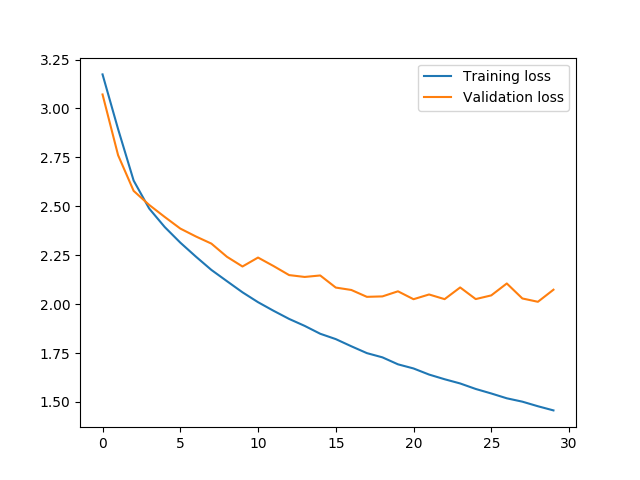
\includegraphics[scale=0.4]{img/norm-loss.png}
    \subcaption{Evolución de la función de pérdida.}
    \label{fig:norm-loss}
  \end{subfigure}%
  ~ \quad
  \begin{subfigure}{.5\textwidth}
  	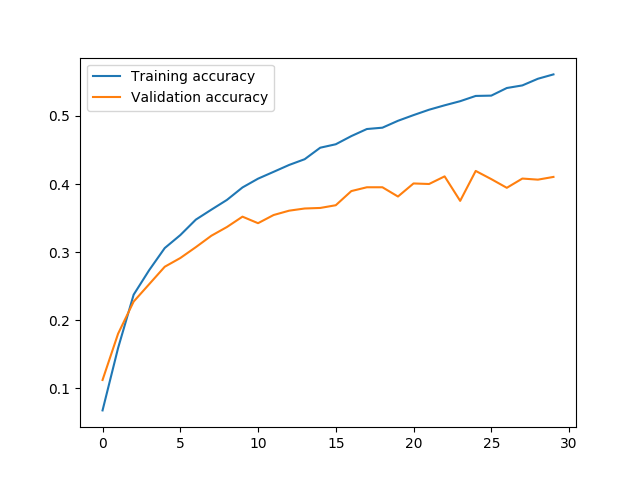
\includegraphics[scale=0.4]{img/norm-acc.png}
  	\subcaption{Evolución de la \textit{accuracy}.}
  	\label{fig:norm-acc}
  \end{subfigure}
  \caption{Historia del modelo \textit{BaseNet} con normalización.}
  \label{fig:norm-history}
\end{figure}

Como podemos ver, comparando los resultados con los que se pueden ver en la figura \ref{fig:basenet-history} los valores de
pérdida son menores en el conjunto de entrenamiento que los que teníamos anteriormente. Además, el valor de \textit{accuracy}
es más alto que el que habíamos obtenido en el caso anterior para el el conjunto de entrenamiento. Sin embargo, si estudiamos
los resultados obtenidos en validación, vemos que no ha habido ninguna mejora significativa, ya que los resultados son bastante
parecidos a los que teníamos anteriormente.

Además de eso, si estudiamos los valores de entrenamiento y de validación de forma conjunta, podemos ver que, a diferencia
de lo que sucedía en la figura \ref{fig:basenet-history}, aquí los resultados en validación se quedan mucho más cortos cuando
llegamos a las últimas épocas. Al principio, los valores van bastante pegados, pero a medida que aumentan el número de épocas,
éstos se van despegando, hasta llegar al resultado final que podemos ver en las gráfias de la figura \ref{fig:norm-history}.

En líneas generales podemos ver que los valores de la función de pérdida en validación se quedan bastante por encima de los de
entrenamiento, y la \textit{accuracy} se queda bastante por debajo de la de entrenamiento. Aparte, en ambos parece que se estanca
en las últimas épocas, mientras que los valores obtenidos en entrenamiento siguen mejorando. Por tanto, podemos detectar cierto
\textit{overfit}, ya que aunque se mejore en entrenamiento, no hay mejoras reales en validación, con lo cuál parece
que el modelo está comenzando a memorizar los datos de entrenamiento. Posiblemente, de haber entrenado algunas épocas más,
los valores de validación hubiesen empezado a empeorar.

Tras este breve análisis podemos ver que, a pesar de que normalizar ha permitido mejorar los resultados obtenidos en entrenamiento,
los de validación aún se quedan muy cortos. Por tanto, ha habido cierta mejora, pero no significativa. Esto puede deberse a que
solo se normaliza la entrada, y a media que se van haciendo convoluciones, dicha normalización se pierde. Con lo cuál, parece
lógico que se tengan que introducir capas de normalización en la red para que los datos siempre estén normalizados, aunque
esto lo haremos más adelante. De momento, conservaremos la normalización, ya que es una mejora que siempre ayuda y, si conseguimos
combinarla con alguna otra mejora, puede que los resultados sean bastante mejores.

\subsection{Aumento de datos}

\subsection{Aumento de la profundidad de la red}

\subsection{Mejora extra: regularización mediante Dropout}

\subsection{Capas de normalización}

\section{\textsc{Transferencia de modelos y ajuste fino con ResNet50 para la base de datos Caltech-UCSD}}

\newpage

\bibliographystyle{plain}
\bibliography{mybib}

\end{document}

